\documentclass{article}

% these packages let you do math
\usepackage{amsmath}
\usepackage{amssymb}

% we need these packages for fancy R tables
\usepackage{booktabs}
\usepackage{float}
\usepackage{colortbl}
\usepackage{xcolor}

% these packages play with the spacing/margins of the document. Uncomment the commands on lines 16 and 17 to see what they do.
\usepackage{a4wide}
\usepackage{setspace}
\usepackage{geometry}
\usepackage{parskip}
%\doublespacing
%\geometry{margin=1.5in}

% this package helps us with including images. Setting the graphics path makes it easier to refer to things in the \includegraphics command.
\usepackage{graphicx}
\graphicspath{ {C:/Users/Haokun Zhang/Desktop/UTexas classes/casual inference/Hidden curriculum/NLSY97_Hidden_Curriculum/figures/} }

% make some hyperlinks using the \href command
\usepackage{hyperref}
\hypersetup{
    colorlinks=true,
    linkcolor=black,
    urlcolor=blue
}

% set the author, title, and date of the document. \maketitle adds it to the document.
\author{Haokun Zhang}
\title{Incarceration Status by Race and Gender in the Year 2002}
\date{Sping 2022}

\begin{document}
\maketitle

\section{Introduction}

In this paper, I summarized the incarceration status by gender and race in 2002. The dataset is from \href{https://www.nlsinfo.org/investigator/pages/search}{NLS investigator}. Among the respondents in 2002, about 97\% of them were not incarcerated in a given month nor in the previous month; 2-3\% were incarcerated previously but not in the given month and 1\% were incarcerated during all or some of them. 
The analyze includes mean numbers of incarceration by race and gender, as well as a linear regression of the effect of gender and race on incarceration. In the regression, the category of Black female is omitted. Constant represents its effect.

The formula of regression is listed below:
$$
    Incarceration in 2002 = {Hispanic}\beta_1 +  {Mixed Race}\beta_2 + {(Non-Black/Non-Hispanic)}\beta_3 + {Male}\beta_4 + \varepsilon
$$

Across selected races, Black male has the highest mean number of Incarceration{\textemdash}around 0.48, it means that black male would spend averagely 0.48 months under incarceration in 2002. Hispanic male has mean incarceration number of 0.15. Mixed Race (Non-Hispanic) female has the third mean incarceration in 2002{\textemdash}around 0.14. 
Figure \ref{incarceration_by_racegender} shows that mean incarceration number of female are significantly lower than male, excepted for Mixed Race (Non-Hispanic) female. In Mixed Race, mean month of male under incarceration is zero. 
Hispanic female's incarceration number is 0.029, Hispanic male will spend about five times higher than female under incarceration. Similar result happens in Non-Black/Non-Hispanic, where male has about 0.11 incarceration number in average and female has 0.019. black female has approximately 0.02, the mean incarceration number of black male is 24 times higher than female. 

\begin{figure}[H]
    \begin{center}
        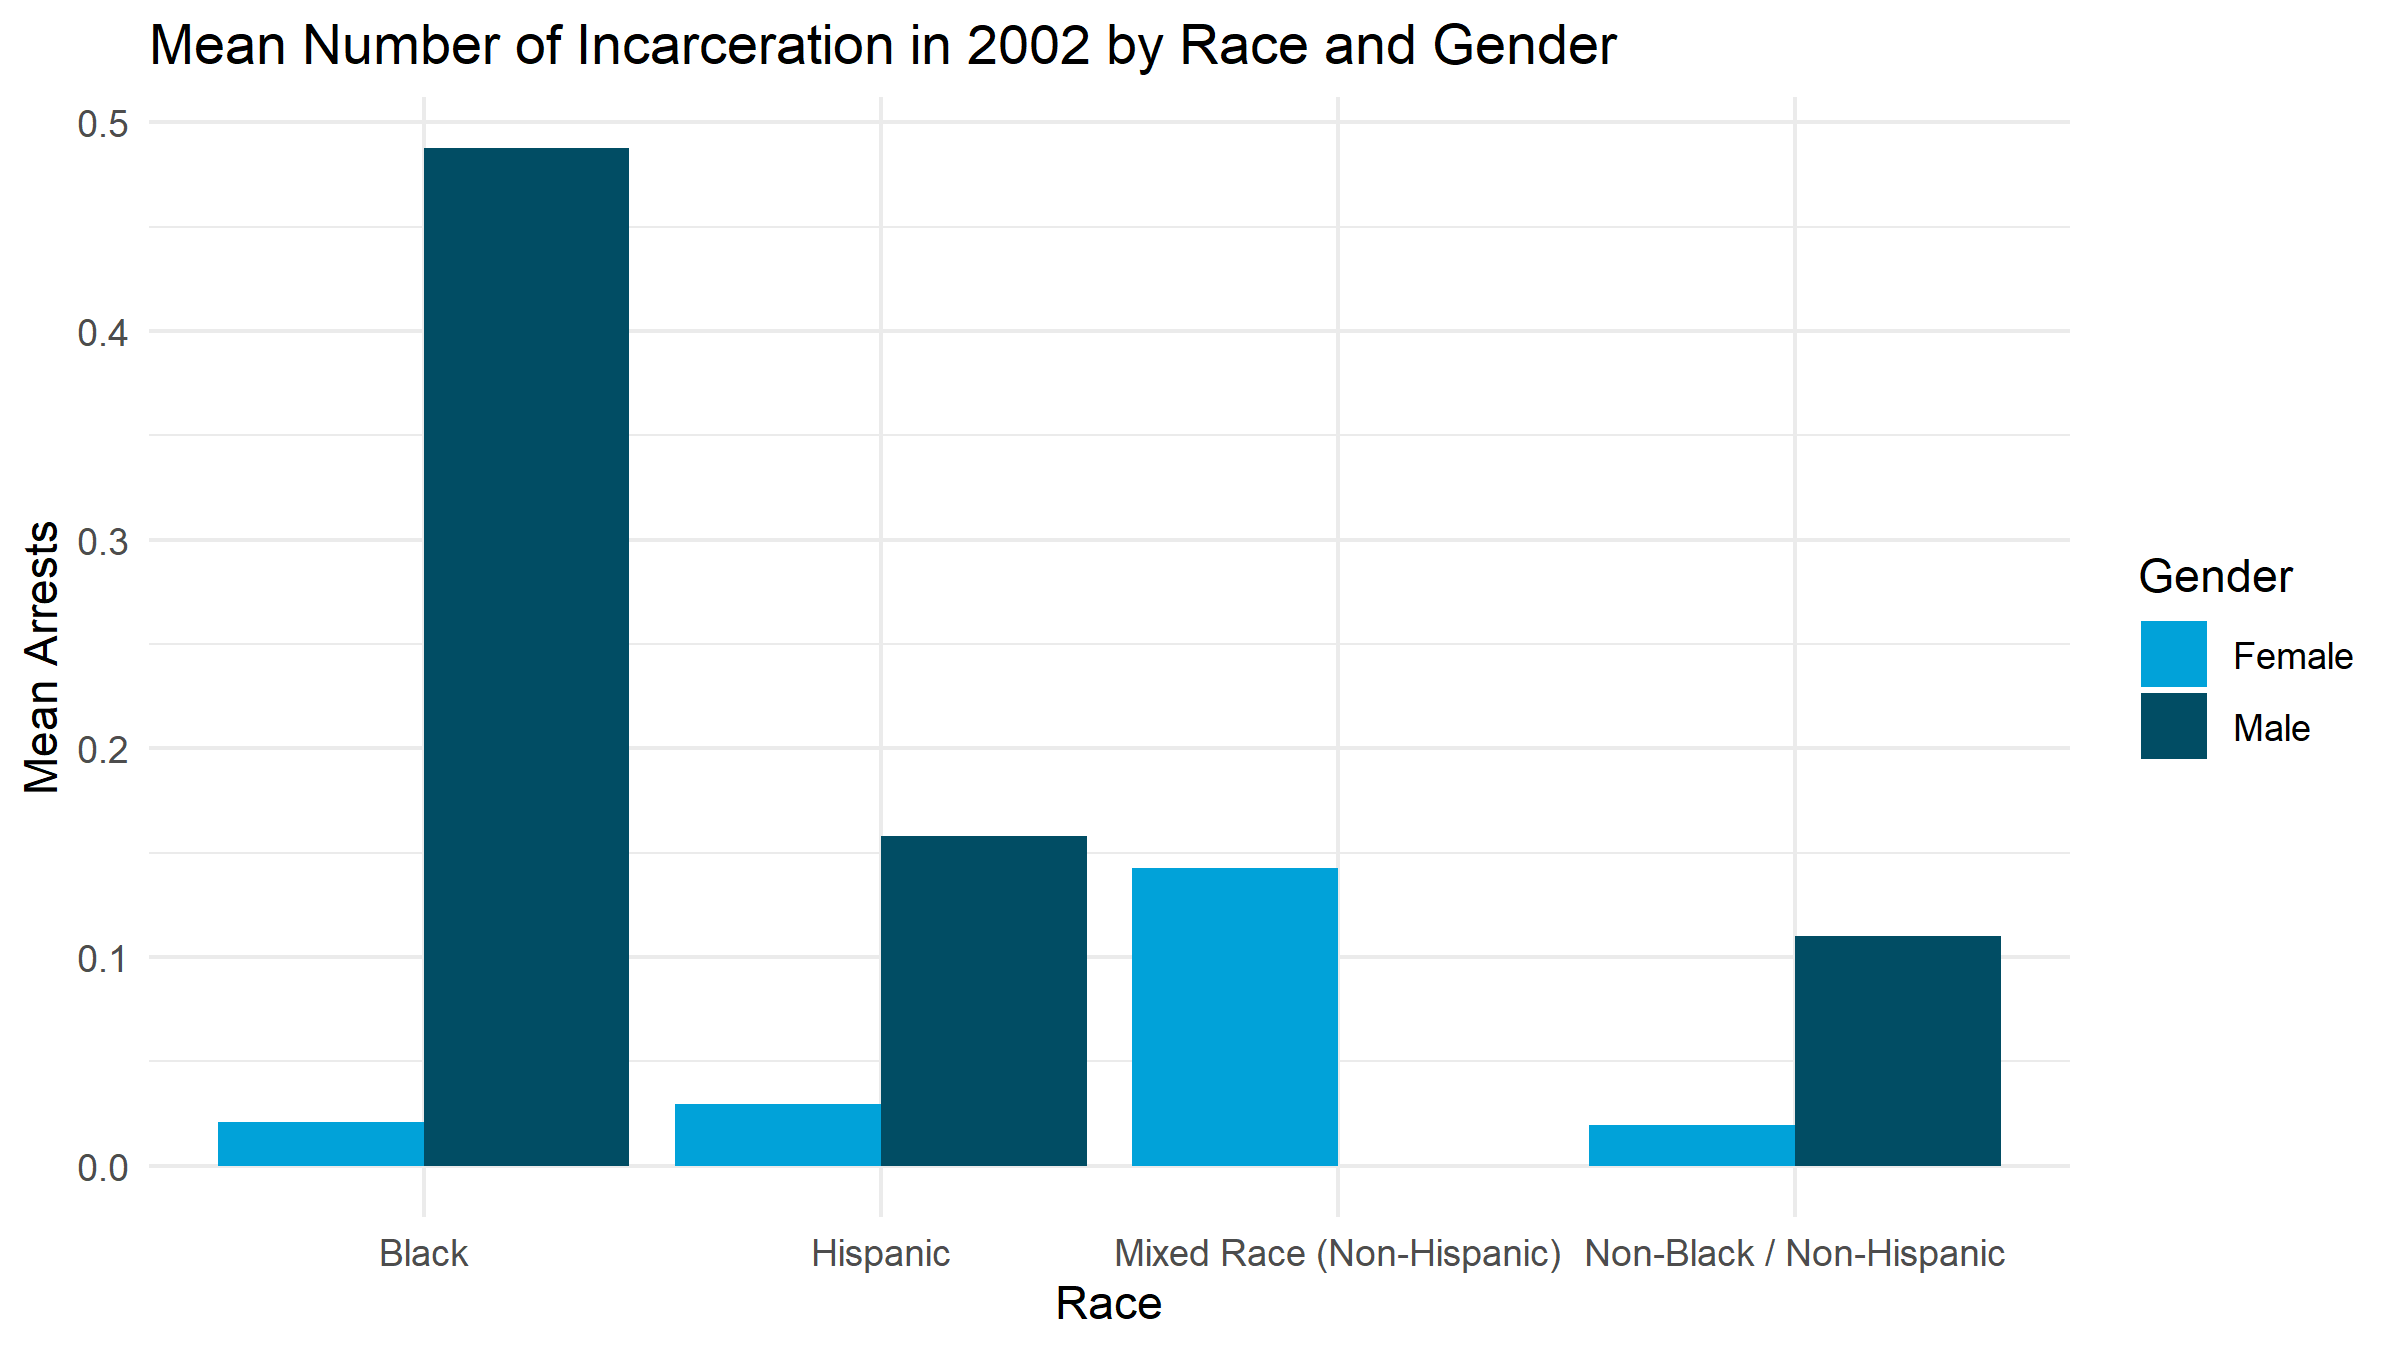
\includegraphics[width=.85\textwidth]{incarceration_by_racegender.png}
    \end{center}
    \caption{Mean Number of Incarceration in 2002 by Race and Gender}
    \label{incarceration_by_racegender}
\end{figure}  

\begin{table}[H]

\caption{\label{tab:tab:summarystats}Mean Incarceration in 2002 by Race and Gender}
\centering
\begin{tabular}[t]{lrrrr}
\toprule
Gender & Black & Hispanic & Mixed Race Non Hispanic & Non Black Non Hispanic\\
\midrule
\cellcolor{gray!6}{Female} & \cellcolor{gray!6}{0.0211268} & \cellcolor{gray!6}{0.0298013} & \cellcolor{gray!6}{0.1428571} & \cellcolor{gray!6}{0.0193192}\\
Male & 0.4876712 & 0.1579509 & 0.0000000 & 0.1099476\\
\bottomrule
\end{tabular}
\end{table}


\newpage

\section{Regression}

Race and gender have impact on incarceration in 2002. Hispanic, Mixed Race (No-Hispanic) and Non-Black/Non-Hispanic decrease the incarceration number, and male gender increases it. Black female also has a positive effect on incarceration.
The three races reduce the incarceration number in similar amount: In 2002, Hispanic would spend 0.159 less months on incarceration; Mixed Race 0.174 and Non-Black/Non-Hispanic 0.189. Male would increase the number by 0.194 and Black female 0.155. All of them are statistically significant at level of 0.01.
It is worth noting that the adjusted R-square value is only 0.014, suggesting that gender and race might have different impact and there are potiently more variables than them having effect on incarceration number. 


% Table created by stargazer v.5.2.2 by Marek Hlavac, Harvard University. E-mail: hlavac at fas.harvard.edu
% Date and time: Fri, Feb 11, 2022 - 3:40:01 PM
\begin{table}[!htbp] \centering 
  \caption{Regression Output. Omitted category is Black Females.} 
  \label{tab:regression} 
\begin{tabular}{@{\extracolsep{5pt}}lc} 
\\[-1.8ex]\hline 
\hline \\[-1.8ex] 
 & \multicolumn{1}{c}{\textit{Dependent variable:}} \\ 
\cline{2-2} 
\\[-1.8ex] & Arrests in 2002 \\ 
\hline \\[-1.8ex] 
 Hispanic & $-$0.159$^{***}$ \\ 
  & (0.038) \\ 
  & \\ 
 Mixed Race (Non-Hispanic) & $-$0.174$^{**}$ \\ 
  & (0.083) \\ 
  & \\ 
 Non-Black / Non-Hispanic & $-$0.189$^{***}$ \\ 
  & (0.035) \\ 
  & \\ 
 Male & 0.194$^{***}$ \\ 
  & (0.022) \\ 
  & \\ 
 Constant & 0.155$^{***}$ \\ 
  & (0.026) \\ 
  & \\ 
\hline \\[-1.8ex] 
Observations & 8,621 \\ 
R$^{2}$ & 0.015 \\ 
Adjusted R$^{2}$ & 0.014 \\ 
Residual Std. Error & 1.019 (df = 8616) \\ 
F Statistic & 32.033$^{***}$ (df = 4; 8616) \\ 
\hline 
\hline \\[-1.8ex] 
\textit{Note:}  & \multicolumn{1}{r}{$^{*}$p$<$0.1; $^{**}$p$<$0.05; $^{***}$p$<$0.01} \\ 
\end{tabular} 
\end{table} 


\newpage

\section{Conclusion}

In this brief analyze of gender and race's impact on incarceration number in 2002, I found that Black male averagely spend more time in jail than other races(Hispanic, Mixed Race and Non-Black/No-Hispanic). Female has much lower incarceration number than male, excepted for Mixed Race. 
Regression result suggests that Hispanic, Mixed Race and Non-Black/Non-Hispanic would reduce the time under incarceration, male and Black female will increase it. 


\end{document}